\chapter{Model-based Reinforcement Learning}
\label{chap4}
\textit{This chapter comprehensively examines the application of data-driven methods to implement \ac{MBRL} for optimal gait control in soft quadruped robots, while also presenting the robot's control architecture.}

\section{Model-based Reinforcement Learning}
The goal of reinforcement learning is to learn a policy that maximizes the cumulative rewards obtained over a sequence of time steps. At each discrete time step denoted by $t$, an agent interacts with its environment. The agent finds itself in a specific state $s_t$ belonging to the state space $S$, then performs an action $a_t$ from the set of possible actions $A$. Following the action, the agent receives an associated reward $r_t$, which depends on the chosen state and action. Afterward, the agent transitions to a new state $s_{t+\Delta t}$, where $\Delta t$ is the time interval between consecutive time steps. These transitions are determined by the underlying, yet unknown, dynamics function $f$, defined as a mapping from pairs of states and actions to subsequent states $f: (s_t, a_t) \rightarrow s_{t+\Delta t}$. 

In the context of \ac{MBRL}, a surrogate model is developed to approximate the dynamics of the environment. This model is employed to predict the future outcomes of actions and states, aiding the agent in making informed decisions. The learned dynamics function is denoted as $\hat{f_\theta}(s_t, a_t)$, and it is parameterized by $\theta$. This learned function accepts the current state $s_t$ and the action $a_t$ as inputs and produces an estimate of the future state $s_{t+\Delta t}$ that the agent will encounter after taking the specified action. The parameter $\theta$ captures the characteristics of the learned function, determining its behavior. In this thesis, the chosen approach involves representing the learned dynamics function $\hat{f_\theta}(s_t, a_t)$ using a deep neural network. This neural network is designed to capture intricate relationships between the input state and action, allowing it to approximate the complex and often nonlinear dynamics of the environment. 

Before initiating the training process, a dataset $D$ was assembled through the collection of training samples. These samples were generated by initializing the system with various starting configurations denoted as $s_0$. Subsequently, random actions $a_t$ were executed at each time step. These actions were drawn from a probability distribution $p(A)$. The outcomes of these actions were recorded, resulting in a sequence of states $(s_0, ..., s_{t-1}, s_t, s_{t+1}, ...)$. In order to ensure uniform treatment of distinct state components, including orientations, velocities, and forces, a preprocessing step is initiated. This involves the subtraction of the mean from the amassed data, succeeded by division by the standard deviation of the dataset, ultimately contributing to the normalization of the data distribution.

\section{Validation}
The surrogate model $\hat{f_\theta}(s_t, a_t)$ was subsequently subjected to a training process employing the dataset $D$. The goal of training was to minimize a specific loss function, specifically half of the \ac{MSE}. The formulation of the loss function is: 
\begin{equation}
    Loss = \frac{1}{|D|}\sum_{(s_t,a_t, s_{t+1}) \in D}^{D} \frac{1}{2}\lVert s_{t+1}-\hat{f_\theta}(s_t, a_t)\rVert^2
\label{eq:loss}
\end{equation} 
Moreover, the \ac{RMSE} was employed to quantify the accuracy of the predictions made by the surrogate model. This metric provides a comprehensive assessment of the residual errors between the predictions and the true values. The \ac{RMSE} is computed as: 
\begin{equation}
    RMSE = \sqrt{\frac{\sum_{D} \frac{1}{2}\lVert s_{t+1}-\hat{f_\theta}(s_t, a_t)\rVert^2}{|D|}}
    \label{eq:RMSE}
\end{equation}
During the training process utilizing the dataset $D$, both the \ac{MSE} and \ac{RMSE} in the aforementioned expressions were computed not only on the training dataset but also on a distinct validation dataset $D_{val}$, which was not part of the training dataset. Additionally, the surrogate model's performance was evaluated on a real-world test gait dataset, denoted as $D_{real}$, employing the \ac{NRMSE}:
\begin{equation}
    NRMSE = \frac{\sqrt{\frac{1}{D_{val}}\sum_{D_{val}}\lVert s_{t+1}-\hat{f_\theta}(s_t, a_t)\rVert^2}}{max(s_t) - min(s_t)}
    \label{eq:NRMSE}
\end{equation}

While these error metrics offer an estimate of the surrogate model's predictive capability for the next state, it is essential to assess its performance in predicting further into the future. This is crucial, as the model will be used for long-horizon control. To this end, the validation errors over a span of T steps were computed. This was achieved by employing the learned surrogate model to make multi-step open-loop predictions. For each given sequence $(a_t, ..., a_{t+T})$ on the initial starting state $s_0$, a comparison was drawn between the corresponding ground-truth states $(s_t, ..., s_{t+T})$ and the multi-step state predictions $(\hat{s_t}, ..., \hat{s_{T}})$ generated by the learned surrogate model. This comparison was formulated as:
\begin{equation}
    NRMSE^{T} = \frac{\sqrt{\frac{1}{D_{val}}\sum_{D_{val}}\frac{1}{T}\sum_{i=1}^{T}\lVert s_{t+i}-\hat{s_{t+i}}\rVert^2}}{max(s_t) - min(s_t)} : 
    \hat{s_{t+i}} = \begin{cases} 
                        s_t & i=0 \\
                        \hat{f_\theta}(s_t, a_t) & i>0
                    \end{cases}
    \label{eq:NRMSET}
\end{equation}
Furthermore, an additional comparison was made between the ground-truth state $(s_{t+T})$ and the state prediction from the last calculated step by the learned surrogate model $(\hat{s_{t+T}})$, incorporating $N$ data:
\begin{equation}
    \rho_{val}^{N} = \frac{\sum_{i=1}^{N}(s_i - \Bar{s_i})(\hat{s_{i}}-\Bar{s_{pred,i}})}{\sqrt{\sum_{i=1}^{N}(s_i - \Bar{s_i})^2 \sum_{i=1}^{N}(\hat{s_{i}}-\Bar{s_{pred,i}})^2}} :
    \Bar{s_{pred,i}} = \frac{1}{n}\sum_{i=1}^{n}\hat{f_\theta}(s_i, a_i)
    \label{eq:R}
\end{equation}
Importantly, the T-step validation procedure was exclusively utilized for result analysis and was not employed during the actual training process.

\section{Neural Networks Design}
When considering the creation of a surrogate model to expedite the RL training process, as discussed in chapter \ref{chap2}, \ac{ANN} come to the forefront of our thoughts due to their inherent capacity to capture complex relationships within data and provide an efficient approximation of underlying dynamics. As highlighted, there exist multiple viable approaches within the realm of \ac{ANN}s, such as typical \ac{DNN}, \ac{RNN} and \ac{CNN}. Although \ac{CNN}  are a subset of feedforward neural networks, their convolutional layers are specifically tailored to discern spatial patterns and features within multidimensional and local receptive fields. This attribute renders them particularly suited for analyzing the influence of actions on subsequent states in a structured manner. However, given that the model at hand pertains to complex temporal relationships, the utilization of \ac{CNN} is not suitable within the scope of this thesis.

Belongs to \ac{ANN}, a typical \ac{DNN} consists of interconnected layers of artificial neurons, including the input layer, hidden layers, and output layer, which builds up the world of artificial intelligence and offers a straightforward design approach. The input layer receives raw data and transfers it to subsequent layers. The hidden layers undertake intermediate computations, employing activation functions to extract intricate features from the data. The output layer produces the final network output based on the assigned task, such as classification or regression. The design of the hidden layers can be meticulously tailored to accommodate various tasks, ensuring adaptability and versatility in tackling diverse computational challenges. 

Emerging as a distinct architecture within the realm of \ac{ANN}, \ac{RNN}s present a distinctive architecture. Setting them apart from the conventional feedforward neural networks, \ac{RNN}s incorporate loops within their structure, thereby enabling the assimilation of sequential and temporal information. This unique characteristic renders \ac{RNN}s especially adept at handling tasks characterized by sequences, time series data, and other dynamic patterns. Notably, each neuron within an \ac{RNN} not only processes the immediate input but also taps into information from preceding time steps, resulting in the creation of an internal memory mechanism. This inherent recurrence empowers \ac{RNN}s to effectively capture dependencies evolving over time and to manage sequences of varying lengths. Given these attributes, \ac{RNN}s are considered a prime choice for capturing the complex dynamics between actions and observations within the SoftQ framework.

\subsection{Neural Network Architecture}
Continuing with the discussion of neural network architecture, it's important to underscore the significance of selecting an appropriate model for the specific task at hand. Commencing with the exploration of the \ac{RNN} architecture, \ac{RNN}s possess a unique characteristic in their design – the inclusion of loops in their architecture. This structural attribute enables them to effectively handle sequential and temporal information, making them particularly well-suited for tasks involving sequences, time series data, and dynamic patterns.
\tikzset{%
  every neuron/.style={
    circle,
    draw,
    minimum size=0.5cm
  },
  neuron missing/.style={
    draw=none, 
    scale=3,
    text height=0.333cm,
    execute at begin node=\color{black}$\vdots$
  },
  rect neuron/.style={ % Define the style for rectangle nodes
  rectangle,
  draw,
  minimum size=0.5cm,
  align=center, 
  },
  cross/.style={
    path picture={
      \draw[black]
        (path picture bounding box.south east) -- (path picture bounding box.north west)
        (path picture bounding box.south west) -- (path picture bounding box.north east);
    }
  },
}

\begin{figure}[ht]
\centering
    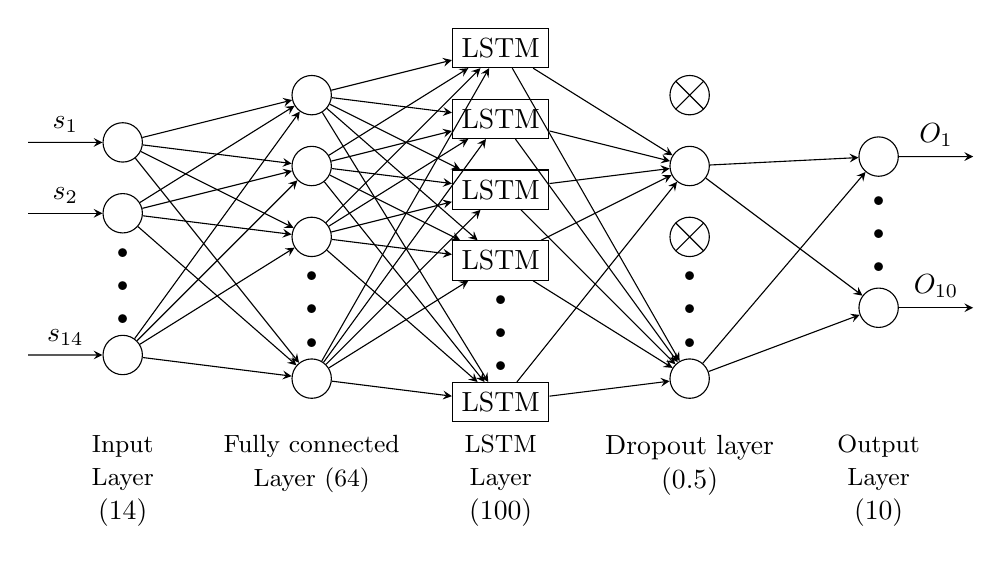
\begin{tikzpicture}[x=1.5cm, y=1.5cm, >=stealth, auto, scale=0.8]
        \foreach \m/\l [count=\y] in {1,2,missing,3}
          \node [every neuron/.try, neuron \m/.try] (input-\m) at (0,2-\y*.75) {};
        \foreach \m [count=\y] in {1,2,3,missing,4}
          \node [every neuron/.try, neuron \m/.try ] (hidden1-\m) at (2,2.5-\y*0.75) {};
        \node [rect neuron/.try, neuron 1/.try] (hidden2-1) at (4,3-1*0.75) {LSTM};
        \node [rect neuron/.try, neuron 2/.try] (hidden2-2) at (4,3-2*0.75) {LSTM};
        \node [rect neuron/.try, neuron 3/.try] (hidden2-3) at (4,3-3*0.75) {LSTM};
        \node [rect neuron/.try, neuron 4/.try] (hidden2-4) at (4,3-4*0.75) {LSTM};
        \node [rect neuron/.try, neuron missing/.try] (hidden2-missing) at (4,3-5*0.75) {};
        \node [rect neuron/.try, neuron 5/.try] (hidden2-5) at (4,3-6*0.75) {LSTM};

        % Dropout Layer
        \node [every neuron/.try, neuron 1/.try ] (dropout-1) at (6,2.5-2*0.75) {};
        \node [every neuron/.try, neuron missing/.try ] (dropout-missing) at (6,2.5-4*0.75) {};
        \node [every neuron/.try, neuron 1/.try ] (dropout-2) at (6,2.5-5*0.75) {};
        \node [every neuron/.try, neuron 1/.try, cross] (dropouted-1) at (6,2.5-1*0.75) {};
        \node [every neuron/.try, neuron 1/.try, cross] (dropouted-2) at (6,2.5-3*0.75) {};
        \foreach \m [count=\y] in {1,missing,2}
          \node [every neuron/.try, neuron \m/.try] (output-\m) at (8,1.9-\y*.8) {};
        \foreach \l [count=\i] in {1,2,14}
          \draw [<-] (input-\i) -- ++(-1,0)
            node [above, midway] {$s_{\l}$};
        \foreach \l [count=\i] in {1,10}
          \draw [->] (output-\i) -- ++(1,0)
            node [above, midway] {$O_{\l}$};
    
        \foreach \i in {1,...,3}
          \foreach \j in {1,...,4}
            \draw [->] (input-\i) -- (hidden1-\j);
        \foreach \i in {1,...,4}
          \foreach \j in {1,...,5}
            \draw [->] (hidden1-\i) -- (hidden2-\j);
        \foreach \i in {1,...,5}
          \foreach \j in {1,...,2}
            \draw [->] (hidden2-\i) -- (dropout-\j);
        \foreach \i in {1,...,2}
          \foreach \j in {1,...,2}
            \draw [->] (dropout-\i) -- (output-\j);
        \foreach \l [count=\x from 0] in {\small Input \\\small Layer\\(14), \small Fully connected \\\small Layer (64), \small LSTM \\\small Layer \\(100), Dropout layer \\(0.5), \small Output \\\small Layer\\(10)}
          \node [align=center, below, yshift=-4.5cm] at (\x*2,2) {\l};
    \end{tikzpicture}
    \caption{\ac{LSTM} \ac{RNN} Architecture. The figure illustrates the architecture of an LSTM-based  RNN. The initial layer comprises the input data, followed by a fully connected layer featuring 64 neurons. Subsequently, the fully connected layer is seamlessly activated by a \ac{ReLU} function before connected to a bidirectional LSTM layer with 100 hidden units. A Dropout layer with 0.5 probability is strategically incorporated before the output layers. }
    \label{fig:lstmstruct}
\end{figure}
        % \foreach \l [count=\i] in {1,2,3,64}
        %   \node [above] at (hidden1-\i.north) {$H_{1,\l}$};
        % \foreach \l [count=\i] in {1,2,3,4,128}
        %   \node [above] at (hidden2-\i.north) {$H_{2,\l}$};
        % \foreach \l [count=\i] in {1,2,3,64}
        %   \node [above] at (hidden3-\i.north) {$H_{3,\l}$};
Each neuron within an \ac{RNN} processes not only the immediate input but also incorporates information from preceding time steps. This intrinsic recurrence empowers \ac{RNN}s to effectively capture and model temporal dynamics, which is crucial for scenarios where actions influence subsequent states over time. As discussed above, the defining characteristic of RNNs lies in their incorporation of loops. These loops create a mechanism by which the output from one step is fed back as an input for the next step. This cyclic connectivity is what allows an RNN to maintain a form of memory across different time steps. In a bit more detail, the RNN takes two main inputs: the current input data and the hidden state from the previous time step. This hidden state is updated through a combination of the current input and the previous hidden state, which are passed through a set of weights and activation functions. Mathematically, the updated hidden state $h(t)$ can be represented as: $h(t) = f(w_i\cdot x(t) + w_j\cdot h(t-1) + w_b)$, where $w_i$ and $w_j$ are the weight metrics, $w_b$ is the bias term and $f$ is the activation function. However, conventional RNNs encounter specific challenges, such as the vanishing gradient problem, which can hinder their ability to effectively learn intricate relationships over extended sequences.

This brings us to the \ac{LSTM} network, an evolved form of the RNN. \ac{LSTM} layers incorporate specialized memory cells and gating mechanisms that enable them to selectively retain or forget information over extended sequences. These mechanisms regulate the flow of information through the network, allowing it to selectively remember or forget information over longer sequences. This makes LSTMs particularly adept at capturing and modeling intricate temporal relationships. Since the surrogate model of SoftQ comprises both past and future context, we have adopted a bidirectional \ac{LSTM} architecture. This entails incorporating two distinct \ac{LSTM} layers. The first layer processes the sequence in the traditional forward direction, while the second layer processes it in reverse. The architecture of the designed bidirectional \ac{LSTM} \ac{RNN} architecture is visually depicted in Fig. \ref{fig:lstmstruct}.

In addition to the \ac{LSTM} layer, incorporating a fully connected layer into the architecture enhances the network's capacity to capture and process complex relationships within sequential data. A fully connected layer, also known as the dense layer, is a fundamental component of neural networks. Each neuron in this layer is connected to every neuron in the previous and subsequent layers, allowing for comprehensive feature extraction and transformation. In fully connected layers, the neuron applies a linear transformation to the input vector through a weights matrix. A non-linear transformation is then applied to the product through a non-linear activation function f: $y_{jk}(x)=f\left(\sum_{i=1}^{n_H} w_{j k} x_i+w_{j0}\right)$. In the end, a dropout layer of 50\% was implemented to enhance the robustness and generalization capabilities of the neural network. A Dropout layer is a regularization technique that aids in preventing overfitting, which randomly sets a portion of the input neurons to zero during training. 
\tikzset{%
  every neuron/.style={
    circle,
    draw,
    minimum size=0.5cm
  },
  neuron missing/.style={
    draw=none, 
    scale=3,
    text height=0.333cm,
    execute at begin node=\color{black}$\vdots$
  },
}

\begin{figure}[ht]
\centering
    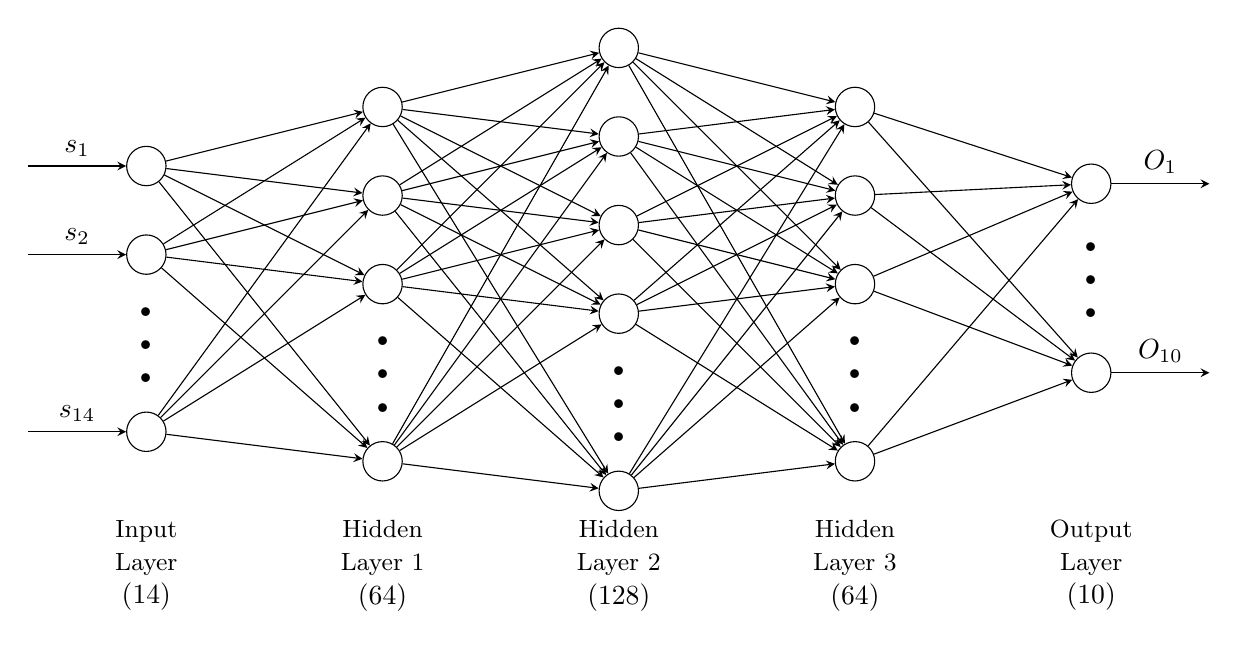
\begin{tikzpicture}[x=1.5cm, y=1.5cm, >=stealth, auto]
    
        \foreach \m/\l [count=\y] in {1,2,missing,3}
          \node [every neuron/.try, neuron \m/.try] (input-\m) at (0,2-\y*.75) {};
        \foreach \m [count=\y] in {1,2,3,missing,4}
          \node [every neuron/.try, neuron \m/.try ] (hidden1-\m) at (2,2.5-\y*0.75) {};
        \foreach \m [count=\y] in {1,2,3,4,missing,5}
          \node [every neuron/.try, neuron \m/.try ] (hidden2-\m) at (4,3-\y*0.75) {};
        \foreach \m [count=\y] in {1,2,3,missing,4}
          \node [every neuron/.try, neuron \m/.try ] (hidden3-\m) at (6,2.5-\y*.75) {};
        \foreach \m [count=\y] in {1,missing,2}
          \node [every neuron/.try, neuron \m/.try ] (output-\m) at (8,1.9-\y*.8) {};
        \foreach \l [count=\i] in {1,2,14}
          \draw [<-] (input-\i) -- ++(-1,0)
            node [above, midway] {$s_{\l}$};
        \foreach \l [count=\i] in {1,10}
          \draw [->] (output-\i) -- ++(1,0)
            node [above, midway] {$O_{\l}$};
        \foreach \i in {1,...,3}
          \foreach \j in {1,...,4}
            \draw [->] (input-\i) -- (hidden1-\j);
        \foreach \i in {1,...,4}
          \foreach \j in {1,...,5}
            \draw [->] (hidden1-\i) -- (hidden2-\j);
        \foreach \i in {1,...,5}
          \foreach \j in {1,...,4}
            \draw [->] (hidden2-\i) -- (hidden3-\j);
        \foreach \i in {1,...,4}
          \foreach \j in {1,...,2}
            \draw [->] (hidden3-\i) -- (output-\j);
        \foreach \l [count=\x from 0] in {\small Input \\\small Layer\\(14) ,\small Hidden \\\small Layer 1\\(64), \small Hidden \\\small Layer 2\\(128), \small Hidden \\\small Layer 3\\(64), \small Output \\\small Layer\\(10)}
          \node [align=center, below, yshift=-5.5cm] at (\x*2,2) {\l};
    \end{tikzpicture}
    \caption{Neural network structure of surrogate model}
    \label{fig:NN}
\end{figure}
        % \foreach \l [count=\i] in {1,2,3,64}
        %   \node [above] at (hidden1-\i.north) {$H_{1,\l}$};
        % \foreach \l [count=\i] in {1,2,3,4,128}
        %   \node [above] at (hidden2-\i.north) {$H_{2,\l}$};
        % \foreach \l [count=\i] in {1,2,3,64}
        %   \node [above] at (hidden3-\i.north) {$H_{3,\l}$};

With the architectural groundwork laid, the bidirectional \ac{LSTM}-based \ac{RNN} embarks on its training journey. During this critical phase, 15\% of the training data was reserved for validation purposes, and the loss and \ac{RMSE} of the training is shown in Fig. \ref{fig:train2net}(a) and (c). Following this validation stage, the network was evaluated with some manual trot gait test data, the evaluation results are shown in Fig. \ref{fig:comp2net}. 

Unlike the sequential and temporal focus of \ac{RNN} models, \ac{DNN} architectures are simpler and characterized by interconnected layers of artificial neurons, with just input, hidden, and output layers. Commencing with the input layer, raw data is received and transmitted to subsequent layers. The hidden layers, positioned between input and output layers, facilitate intermediate computations. These computations are facilitated by the application of activation functions between each hidden layers, with the \ac{ReLu} activation function being utilized in this instance. \ac{ReLu} introduces non-linearity by transforming negative values to zero and leaving positive values unaltered through element-wise activation. Finally, the output layer generates the final network output, tailored to the designated regression task. The architecture is visually articulated in Fig. \ref{fig:NN}, offering a tangible representation of the underlying structural arrangement. 

\subsection{Optimization Algorithms}
Furthermore, it is essential to emphasize that alongside architectural considerations, the choice of optimization algorithms holds significant importance before the commencement of the training process. These algorithms steer the iterative parameter updates that guide the model towards convergence. Popular optimization algorithms include \ac{SGDM}, \ac{Adam}, and \ac{RMSProp}. These algorithms adjust the weights of the model based on the gradients of the loss function with respect to the parameters. They help to guide the model towards finding optimal parameter values that minimize the loss function.

\ac{SGDM} augments the standard Stochastic Gradient Descent (SGD) by introducing a momentum term. This term incorporates the weighted average of the previous gradients to determine the direction of the parameter updates. This addition imparts momentum to the optimization process, allowing for smoother convergence by reducing the oscillations that can occur during gradient updates. The momentum term helps to accelerate the movement along shallow directions while dampening oscillations in steep directions. 

\ac{Adam} is an optimization algorithm that combines the advantages of both momentum-based methods and adaptive learning rates. It maintains exponentially decaying moving averages of both past gradients and past squared gradients. These moving averages are used to compute adaptive learning rates for individual parameters. Additionally, \ac{Adam} employs bias correction mechanisms to counteract potential bias towards zero at the beginning of training. By adjusting the learning rates dynamically based on the historical gradients, \ac{Adam} enhances convergence speed and adaptability across varying gradients.

\ac{RMSProp} is an optimization technique designed to address the challenges of learning rate selection in \ac{SGDM}. It maintains an exponentially decaying average of squared gradients for each parameter. The learning rate is then divided by the square root of this average, which normalizes the learning rate by the historical gradient magnitudes. This adaptive learning rate adjustment helps to mitigate the problem of diminishing or exploding gradients.

\begin{figure}[htb]
    \centering
    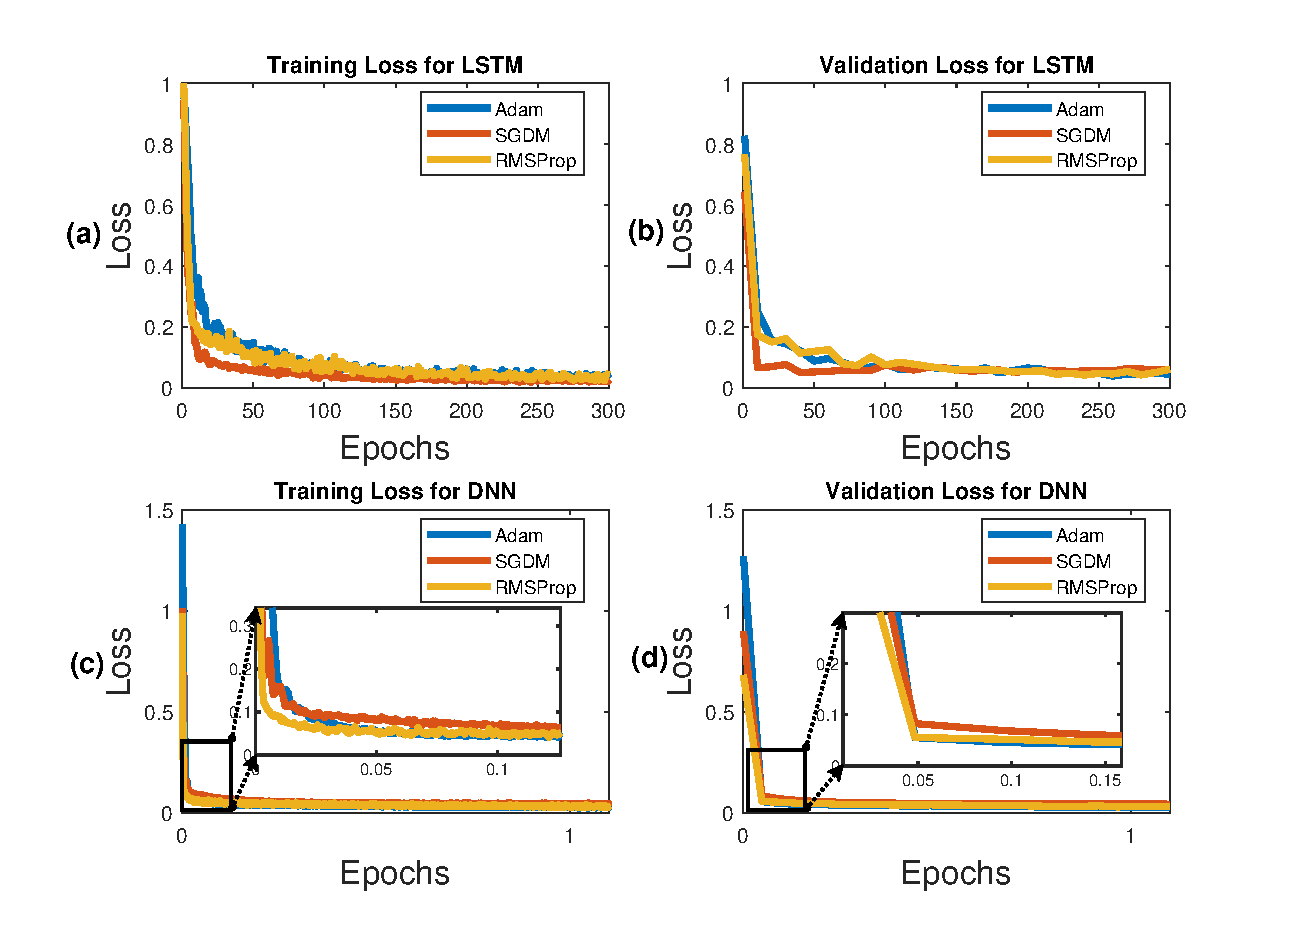
\includegraphics[width=\linewidth]{img/chap4/comp_op.eps}
    \caption{Comparison of Training Trajectories with Different Optimization Algorithms. The figure illustrates the training trajectories of two applied architectures while employing three different optimization algorithms: \ac{SGDM}, \ac{Adam}, \ac{RMSProp}. (a) Training loss and (b) validation loss for the bidirectional \ac{LSTM}-based \ac{RNN} architecture, (c) training loss (d) validation loss for the \ac{DNN} architecture.}
    \label{fig:comp3op}
\end{figure}

By implementing all three optimization algorithms in two networks, a comprehensive exploration was undertaken to discern the most suitable optimization strategy for the training of the surrogate model. This comprehensive approach facilitated a comprehensive assessment of each algorithm's impact on the training process and subsequent model performance. Specifically, the training was performed on both the bidirectional LSTM-RNN and DNN architectures, maintaining a consistent learning rate of 0.001. The training data was shuffled at the end of each epoch, and a mini-batch size of 512 was utilized. The training trajectories of the bidirectional LSTM-RNN and DNN networks, encompassing the utilization of the three optimization algorithms, are visually depicted in Figure \ref{fig:comp3op}. 

For the bidirectional LSTM-based RNN architecture, SGDM is the emerged as the optimal choice due to its remarkable ability to achieve the lowest training loss and converge rapidly. It exhibited both the fastest convergence and the least training loss among the evaluated optimization algorithms. In contrast, for the DNN architecture, took the lead. Adam demonstrated superior performance by learning rapidly and converging to the lowest loss values, both in validation and training. Its ability to efficiently navigate the DNN's training dynamics underscores its suitability for this architecture. Notably, all three optimization algorithms proved to be stable options for training this architecture effectively.

\subsection{Network Validation}
\begin{figure}[htb]
    \centering
    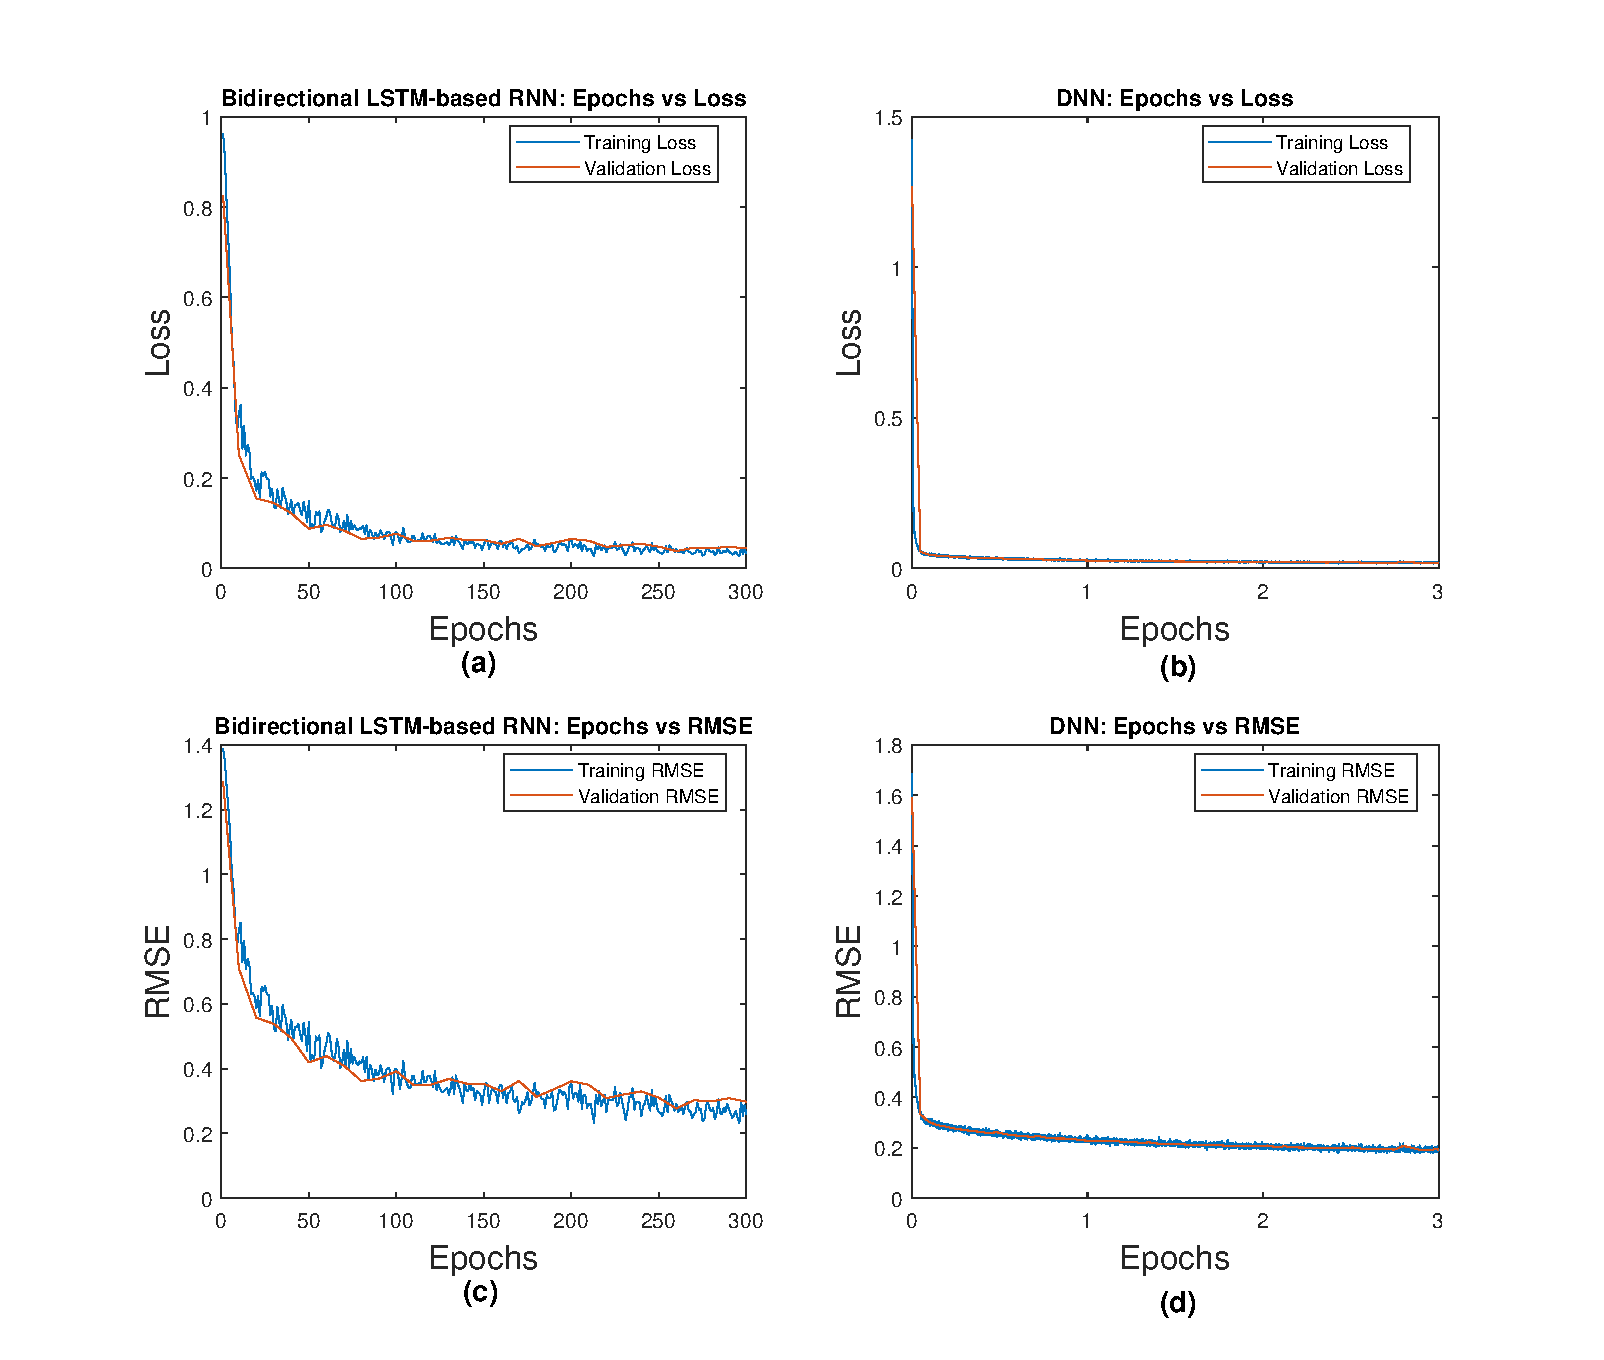
\includegraphics[width=\linewidth]{img/chap4/train_result.eps}
    \caption{Training of bidirectional LSTM-RNN architecture and DNN architecture. (a)-(b) Loss vs epoch for model training with bidirectional LSTM-based and DNN model; (c)-(d) RMSE vs epoch for model training with bidirectional LSTM-based and DNN model.}
    \label{fig:train2net}
\end{figure}

Nonetheless, when comparing the training performance of the bidirectional LSTM-based RNN architecture and the DNN architecture, as illustrated in Figure \ref{fig:train2net}, it becomes evident that the DNN architecture exhibits greater efficiency in terms of data utilization. Notably, the DNN showcases the capability to converge to a lower loss while achieving a reduced \ac{NRMSE}. This underscores the DNN's efficiency in leveraging the provided data and achieving enhanced predictive accuracy with a more compact loss function. Furthermore, evaluated against the real expert trot gait simulation data, the bidirectional LSTM-based RNN architecture achieves an NRMSE of approximately 0.82 for single step prediction, whereas the DNN attains a significantly lower NRMSE of around 0.26. This substantial divergence in NRMSE values highlights the DNN's proficiency in making more accurate predictions on these test cases. A more comprehensive review of the single-step predictions, as compared to the expert trot simulation data, can be observed in Figure \ref{fig:lstm_test} and Figure \ref{fig:DNN_test} in the Appendix. 

\begin{figure}[htb]
    \centering
    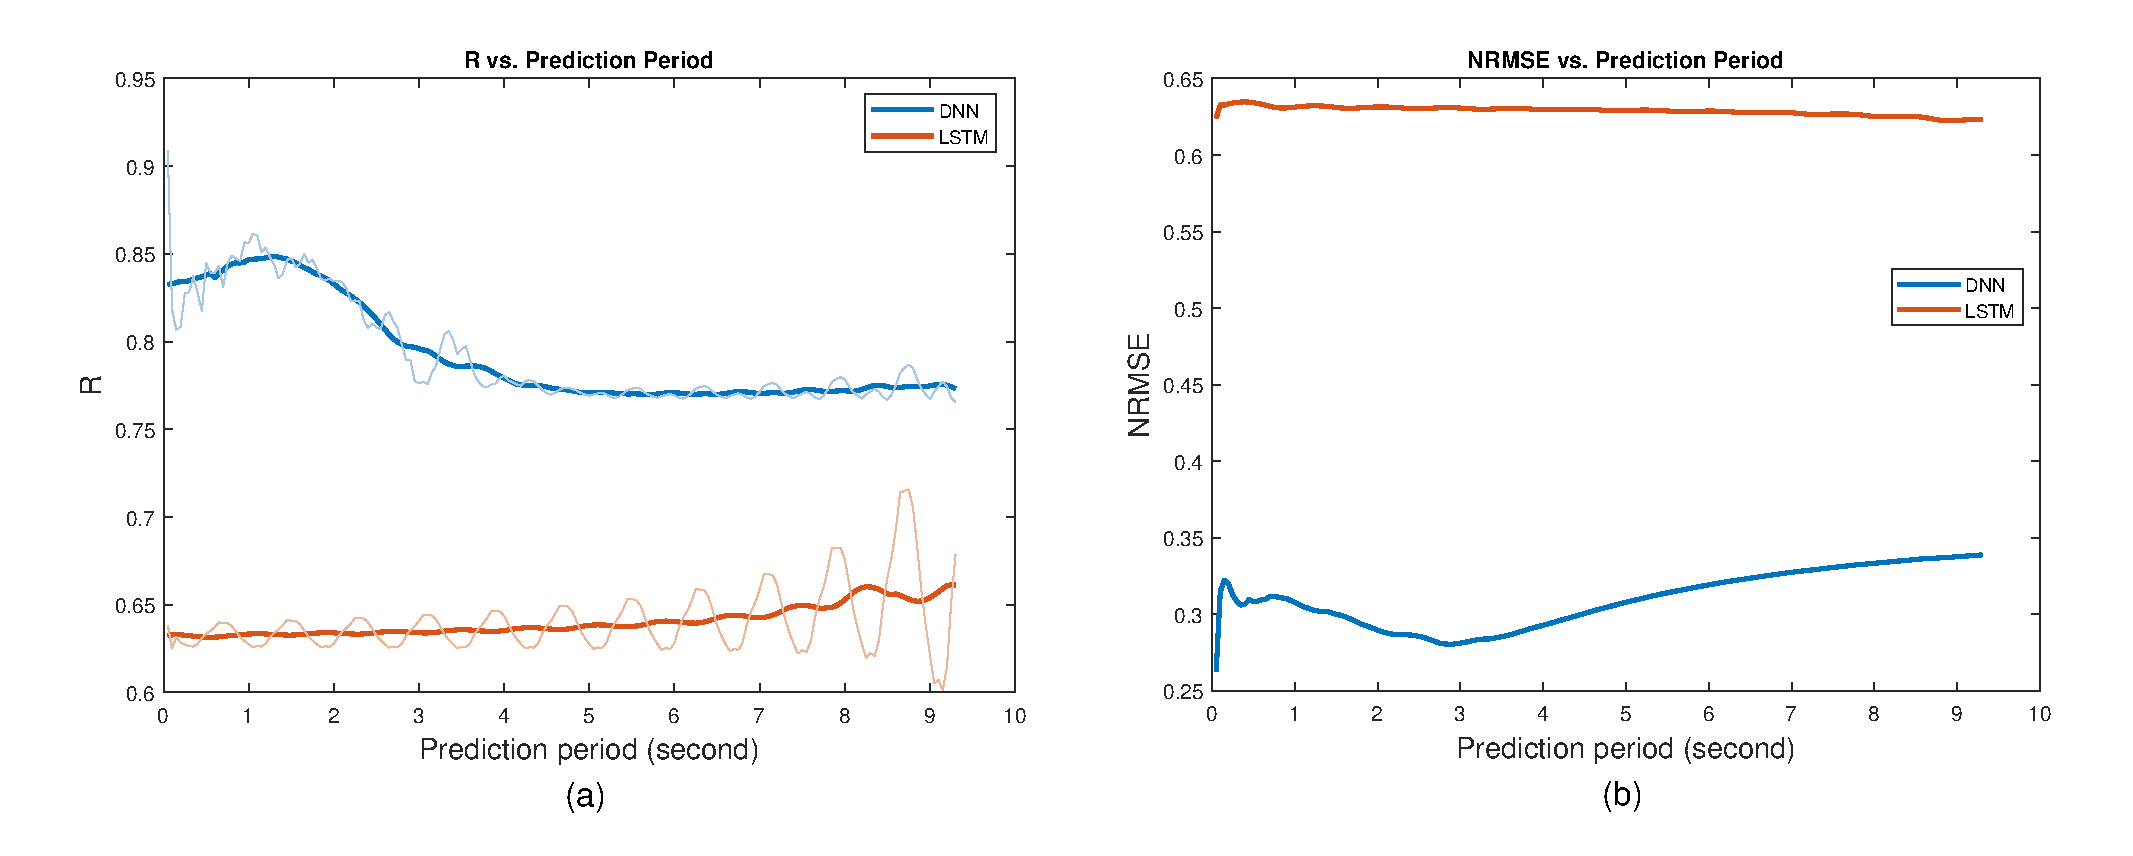
\includegraphics[width=0.9\linewidth]{img/chap4/long2net.eps}
    \caption{Comparison of Long-Term Predictions using some Expert Trot Gait Data. The figure illustrates the average correlation coefficient (R) of long-term predictions between the DNN architecture and the bidirectional LSTM-based RNN architecture.}
    \label{fig:comp2net}
\end{figure}

In addition, an evaluation of the long-term predictions produced by both architectures, as illustrated in Figure \ref{fig:comp2net}, reveals valuable insights. The average correlation coefficient (R) of DNN architecture's single-step predictions surpasses 0.9, and it maintains a commendable level of above 0.76 for predictions spanning 10 seconds. On the other hand, the bidirectional LSTM-based RNN architecture demonstrates a single-step correlation coefficient (R) of around 0.74, indicating its ability to predict long-term and time-series data with consistency. However, it's worth noting that this correlation coefficient (R) does not exhibit substantial enhancement for longer prediction horizons, setting it apart from the DNN architecture. In light of these comparisons and insights, the DNN architecture optimized with the Adam optimization algorithm emerges as a promising choice for surrogate model training.


\subsection{Dataset Size}
The neural network's architecture, as discussed earlier, provided the framework for representing the complex relationships within the soft quadruped robot's behavior. However, the size of dataset remains a critical factor in enabling the neural network to learn effectively and achieve high estimation accuracy. A dataset of sufficient size is essential to provide the neural network with a diverse range of examples that span various scenarios and conditions. This diversity enables the network to generalize well and effectively capture the underlying relationships present in the soft quadruped robot's dynamics. A small dataset might lead to overfitting, where the network memorizes the training examples without truly understanding the underlying patterns. On the other hand, a larger dataset helps the network learn the underlying patterns more comprehensively and reduces the risk of overfitting. 

Furthermore, a larger dataset contributes to improved generalization, enhancing the network's ability to accurately estimate the behavior of the soft quadruped robot across a wider range of situations, even those it hasn't encountered during training. This is particularly important when deploying the surrogate model in real-world scenarios where the conditions might vary.

However, it's crucial to strike a balance between dataset size and the associated computational resources and time required for training. Collecting and curating a substantial dataset demands significant effort and resources, and training a neural network on a large dataset can be computationally intensive. Therefore, careful consideration is required to determine an appropriate dataset size that aligns with the available resources while still achieving the desired level of accuracy and generalization.

\section{Model-based RL Algorithm}
After successfully training the surrogate model, the next phase of this thesis involves the application of \ac{MBRL} algorithms to further advance our research objectives. As previously discussed in Chapter \ref{chap2}, the \ac{SAC} algorithm has been selected due to its advantages in promoting efficient exploration and its compatibility with continuous action spaces. These attributes make SAC a suitable choice for learning and optimizing the optimal gait control strategies for the soft quadruped robot.

SAC is an established RL algorithm that combines key elements from both actor-critic methods and maximum entropy reinforcement learning. The central objective of SAC is to derive a policy that maximizes the cumulative expected reward while also taking into account the entropy of the policy distribution. This dual consideration fosters effective exploration, enabling the algorithm to discover a diverse range of potential control strategies.

By employing SAC, the soft quadruped robot can autonomously learn the optimal gait control strategy through interaction with its environment. The algorithm takes into account the dynamics learned from the surrogate model and uses this information to make informed decisions that lead to better performance in terms of gait control. This step serves as a crucial bridge between the surrogate model training and the practical application of the learned knowledge in a real-world scenario.

The servo motors receive \ac{PWM} signals generated by the control software, which translate to specific rotational torques applied to the actuators. These torques cause the deformation of the actuators, resulting in controlled limb motions that facilitate different gaits. The details of control architecture and the model-based reinforcement learning framework will be shown in the next chapter. To achieve this, the MBRL algorithm is implemented on a high-performance computing system, which interfaces with the robot through the electrical interface board. This system demonstrates the training process and execution of control policies, establishing a bidirectional communication link with the robot for real-time data exchange. For accurate pose and localization feedback, the \ac{IMU} sensor, complemented by the \ac{ToF} sensors, continuously measures the robot's orientation and distance from surrounding objects. This sensory input is processed by the control software to generate state information for the MBRL algorithm.


\section{Control architecture Design}
\begin{figure}[htb]
    \centering
    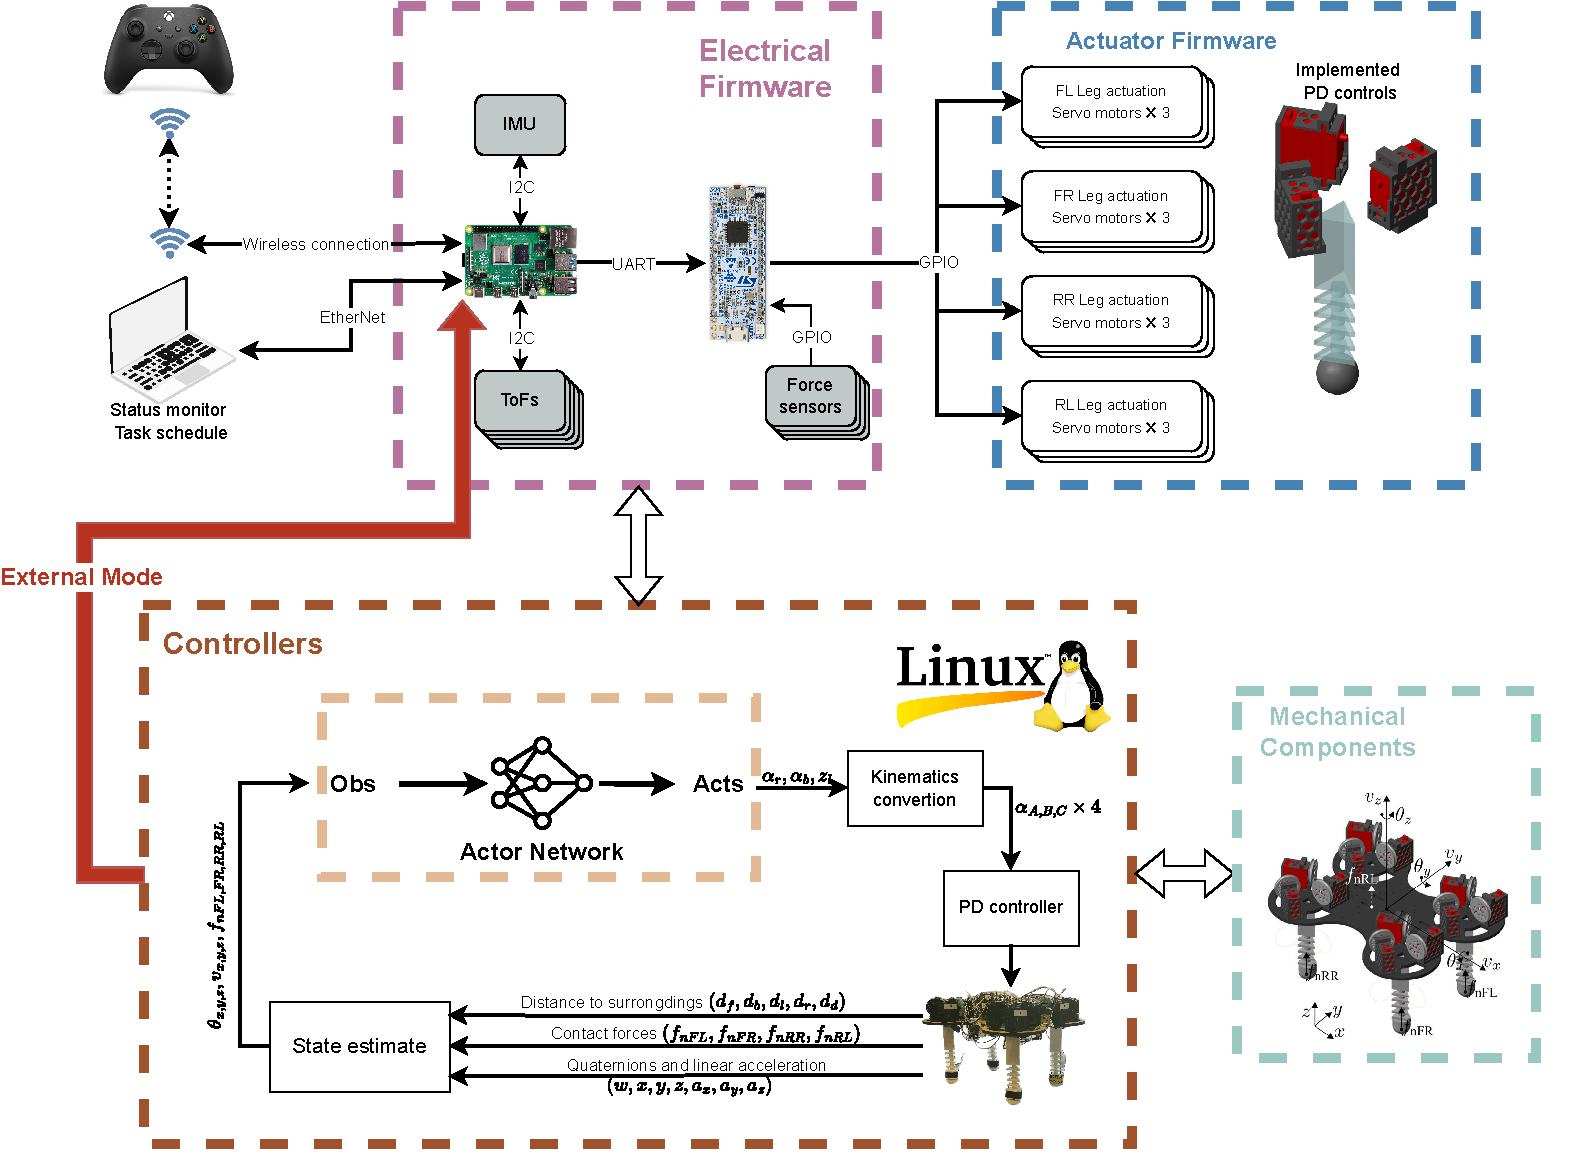
\includegraphics[width=\linewidth]{img/chap4/control.pdf}
    \caption{Graphical overview of control architecture of SoftQ.}
    \label{fig:control}
\end{figure}

\subsection{Task Planning and Execution}

Even though euler angles are used to represent rotations, the transmission of two poses are calculated by Quaternion, which is a mathematical construct that extends the notion of complex numbers to four dimensions. They comprise four components: a scalar part represented by $w$, and a vector component denoted as $\vec{v}=(x, y, z)$. Quaternions are expressed as:
$$q = w + xi + yj + zk$$
where $x$, $y$, $z$, and $w$ are real numbers, and $i$, $j$, and $k$ are three imaginary units that satisfy the following multiplication rules: $i^2 = j^2 = k^2 = ijk = -1$. This approach involves establishing the initial pose of the robot as a quaternion and subsequently obtaining the current pose through sensors like accelerometers and gyroscopes. By computing the change in pose between the initial and current states, the rotational component can be extracted. This rotational component provides insights into the rotation axis and angle. To determine the robot's velocity, differentiation of the position component in the current pose is performed with respect to time. The resultant velocity vector is then transformed into the world coordinate frame, leveraging the robot's current orientation. This computation culminates in the derivation of the angular velocity vector and the linear velocity vector, which serve as the final outcomes of this process. Eventually, with all subsystems modeled, the quadruped robot system is assembled and simulated in the MATLAB Simscape environment.

\subsection{Potential Reality Gap}
Transitioning to a different facet of consideration, it's crucial to address the concept of the "Potential Reality Gap." In the realm of reinforcement learning, the surrogate model serves as a bridge between simulation environments and real-world scenarios. However, due to the inherent complexity and uncertainty associated with real-world environments, a misalignment often arises between the training data collected from simulations and the actual performance of the trained model in real-world situations. This discrepancy is referred to as the "Reality Gap."

The Reality Gap poses a challenge because the surrogate model might perform exceptionally well during training in simulation environments but struggle to generalize effectively to real-world settings. This phenomenon can stem from several factors, including variations in physical dynamics, sensor noise, and unmodeled environmental influences. To address the Reality Gap, certain strategies can be adopted. One approach involves introducing stochasticity during training in simulations, simulating uncertainties and disturbances that are characteristic of real-world scenarios. This helps the model develop robustness to unexpected variations.